%   MSc Business Analytics Dissertation
%   Format based on skeleton template provided as part of module MIS40750
%
%   Title:     Optimising the design of buffer preparation in bioprocessing
%              facilities
%   Author:    Sean Tully
%
%   Chapter 4: Methodology
%
%   Change Control:
%   When     Who   Ver  What
%   -------  ----  ---  --------------------------------------------------------
%   06Jun16  ST    0.1  Begun
%

\chapter{Methodology}\label{C.methodology}

\begin{quote}
Just as the largest library, badly arranged, is not so useful as a very
moderate one that is well arranged, so the greatest amount of knowledge, if not
elaborated by our own thoughts, is worth much less than a far smaller volume
that has been abundantly and repeatedly though over.  For only by universally
combining what we know, by comparing every truth with every other, do we fully
assimilate our own knowledge and get it into our power.

\hspace{2cm}--- Arthur Schopenhauer, \emph{On Thinking for Oneself}
\end{quote}

\section{Introduction}\label{S.intro4}

At first glance, the pathway to solving the vessel selection problem was
unclear.
There are two aspects to the problem; scheduling and selection.
The selection problem appears to be a close relative of a number of classic
\textbf{NP}-hard problems in the ``bin-packing'' genre.
For the scheduling aspect of the problem, initial concepts involved finding an
API to one of the commercial scheduling packages.
One initial concept included developing an algorithm to intelligently guess
possible vessel selections, and pass these into a scheduling model which
could be repeatedly be solved using a commercial scheduling package
to find an optimum selection.

On completion of the module on linear programming, it became apparent that
many bin-packing type problems are most efficiently solved using linear
programming techniques.
Additionally, linear programming could be used to model scheduling constraints.

The vessel selection problem was thus formulated as a MILP problem.
Firstly, the problem was described mathematically.
Next, attention was focused on the method of solution.
There are many available linear programming solvers, both proprietary and open
source.
Many proprietary solvers have free academic licenses.
The XPRESS solver from FICO was familiar to the author from the course module
in linear programming, but the documentation is poor and the licensing system
required connection to university servers which proved unreliable remotely.
The version available through the university also had no python API (one is
available in more recent versions), which was a strong preference for output
data analysis and plotting.

The CPLEX solver from IBM was investigated.
The quality of the documentation is excellent, and there is a full python API
which also has excellent documentation.

The MILP problem was thus constructed in python and then solved via the CPLEX
python API.
It was apparent that comparatively few lines of the code involved interface
with the API.
With a view to making this research as useful as possible, open-source
alternatives were also investigated.
In the end, the PuLP python library was used as a bridge between problem
generation and problem solution.
PuLP is an open-source python library which acts as an API to several
(MI)LP solvers, both commercial and open source, allowing the possibility of a
fully open-source tool-chain for solving the problem.

\section{Slots}\label{S.slots}

To model the problem as an MILP problem, we must introduce the concept of
\emph{slots}.
Noting that there is a buffer hold vessel for each buffer, it is evident that
a feasible but inefficient solution could involve installing a dedicated,
suitably sized, preparation vessel for each hold vessel.
Any solution involving more than this number of preparation vessels would not
be optimal.
As a result, we have an upper limit of $\mathcal{N}$ on the number of required
preparation vessels.
The model is thus constructed with $\mathcal{P}$ \emph{slots}, where
\begin{equation}
    \mathcal{P} = \mathcal{N}
\end{equation}
A slot, $p \in P$ is a notional space which may be occupied by a vessel, or may
be empty.
\begin{equation}
    p \in P; \quad P = \left\{ 0, 1, 2, \ldots, p, \ldots, \left( 
    \mathcal{P} - 1 \right) \right\}
\end{equation}
Note that slots do not have any physical significance, i.e. in a real-world
facility, floor space is assigned to physical vessels, rather than notional
slots.

\section{Objective Function}\label{S.objfn}

The vessel selection problem may be described as a series of linear
constraints.
These constraints are applied to find the optimum value of an objective
function, which we seek to minimise.
The primary objective function is the total cost of vessels.
We find this by summing the vessel costs for all vessels present in slots.
Recall that the vessel data set contains entries for $\mathcal{M}$ vessel
sizes, each of which has an associated cost, $c_{m}$.

We now introduce the first decision variable, $\boldsymbol{y}_{mp}$.
This a binary decision variable with dimensions
$\mathcal{M} \times \mathcal{P}$.
Note that binary decision variables may only take the values 0 and 1, i.e.
\begin{equation}
    \boldsymbol{y}_{mp} \in \left\{ 0, 1 \right\} \quad \forall m \in M \quad
    \forall p \in P
    \label{eq.y}
\end{equation}
The possible states of $\boldsymbol{y}_{mp}$ may be described thus:
\begin{equation}
    \boldsymbol{y}_{mp} =
    \begin{cases}
        1 \implies \text{instance of vessel $m$ in slot $p$}\\
        0 \implies \text{otherwise}
    \end{cases}
\end{equation}
We can now describe the objective function, which gives the objective function
value, $\boldsymbol{Z}$.  The objective is to minimise $\boldsymbol{Z}$.
\begin{equation}
    \boldsymbol{Z} = \sum_{m \in M} \sum_{p \in P} c_m \boldsymbol{y}_{mp}
    \label{eq.objfn}
\end{equation}

\section{Basic Model}\label{S.basicprob}

A small number of constraints need to be applied to arrive at the simplest
variant of the problem.
Additional constraints may then be added to make the model more detailed or
realistic.

\subsection{Buffers Dedicated to Slots}\label{SS.constr1}

The first constraint to be added is the limitation that a buffer must be
prepared in exactly one slot.
This constraint means that we must prepare each buffer once per cycle
and also that the buffer is always prepared in the same slot, i.e. slot
selection for every cycle is identical.

We introduce a new binary decision variable, $\boldsymbol{x}_{np}$, which takes
a value of 1 if buffer n is prepared in slot p, and takes a value of 0
otherwise, i.e.
\begin{equation}
    \boldsymbol{x}_{np} \in \left\{ 0, 1 \right\} \quad \forall n \in N \quad
    \forall p \in P
    \label{eq.x}
\end{equation}
Note that $\boldsymbol{x}_{np}$ has dimensions of
$\mathcal{N} \times \mathcal{P}$.
The possible states of $\boldsymbol{x}_{np}$ may be described thus:
\begin{equation}
    \boldsymbol{x}_{np} =
    \begin{cases}
        1 \implies \text{buffer $n$ prepared in slot $p$}\\
        0 \implies \text{otherwise}
    \end{cases}
\end{equation}
The following constraint can now be defined:
\begin{equation}
    \sum_{p \in P} \boldsymbol{x}_{np} = 1 \quad \forall n \in N
    \label{eq.constr1}
\end{equation}

\subsection{Vessel Instances Dedicated to Slots}\label{SS.constr2}

The second constraint to be added is the requirement that at most one vessel
may inhabit a given slot.
This is not directly analogous to the first constraint; it is possible to
use the same \emph{sized} vessel in many slots, but a maximum of one vessel
\emph{instance} may inhabit any given slot.
Note that this inequality allows for the possibility of unused slots, i.e. the
number of occupied slots (and hence the number of preparation vessels) may be
less than the number of available slots (and hence the number of buffers).
\begin{equation}
    \sum_{m \in M} \boldsymbol{y}_{mp} \le 1 \quad \forall p \in P
    \label{eq.constr2}
\end{equation}

\subsection{Vessel Capacity}\label{SS.constr3}

The third constraint is the requirement that, if a vessel is in a given slot,
it has an appropriate volume to prepare all buffers assigned to the slot.
There are two facets to the above statement.
Firstly, we cannot produce buffer volumes greater than the preparation vessel
maximum working volume.
Additionally, vessels have a minimum fill ratio, $r_{MINFILL}$, usually in the
range 10 - 30 \%.
The minimum fill ratio is generally a function of the minimum stir volume of a
vessel's impeller.

More complicated rules may be applied, such as the ability to make an excess
of buffer to prevent the requirement for adding a smaller vessel, but such
approaches are beyond the scope of this basic model.

Recall that for each vessel size, $m \in M$, we have defined a (maximum) vessel
volume, $V_{m}$. Also, for each buffer, $n \in N$, we have defined the required
volume, $U_{n}$.

The maximum vessel capacity constraint is:
\begin{equation}
    U_{n} \boldsymbol{x}_{np} - \sum_{m \in M} V_{m} \boldsymbol{y}_{mp} \le 0
    \quad \forall n \in N, \quad \forall p \in P
    \label{eq.constr3a}
\end{equation}
The minimum vessel capacity constraint is slightly more complex, in that the
\emph{big-M} method must be utilised. The value used for \emph{big-M} is
$V_{\mathit{MAX}}$, where:
\begin{equation}
    V_{\mathit{MAX}} = \text{max} \left( V_{m} \quad \forall m \in M \right)
\end{equation}
The minimum vessel capacity constraint is defined as:
\begin{equation}
    V_{\mathit{MAX}} \boldsymbol{x}_{np} + r_{\mathit{MINFILL}} \sum_{m \in M}
    V_{m} \boldsymbol{y}_{mp} \le U_{n} + V_{\mathit{MAX}} \quad \forall n \in
    N, \quad \forall p \in P
    \label{eq.constr3b}
\end{equation}

\subsection{Preparation Vessel Utilisation}\label{SS.constr4}

In the absence of detailed scheduling data (i.e. knowledge of when the buffers
are used by the process and their durations of use), an allowance can be made
for unknown scheduling constraints by limiting the maximum allowed utilisation
of the preparation vessels.
Note that this will result in a crude approximation but it is often the case
that detailed timing information is not available or cannot be predicted with
sufficient accuracy.
We thus introduce the parameter $r_{\mathit{UTIL}}$, the maximum utilisation
ratio.
The total duration of all preparation procedures in a given slot must not be
above $r_{\mathit{UTIL}} \lambda$, where $\lambda$ is the cycle time of the
process.

The total duration of a single preparation procedure,
$\Delta t_{\mathit{PREP,TOTAL}}$, is given by:
\begin{equation}
    \Delta t_{\mathit{PREP,TOTAL}} = \Delta t_{\mathit{PREP,PRE}} + 
    \Delta t_{\mathit{TRANSFER}} + \Delta t_{\mathit{PREP,POST}}
\end{equation}
Note that, for the basic case, it is only strictly necessary to know
$\Delta t_{\mathit{PREP,TOTAL}}$; the constituent durations do not need to be
known individually.

The following constraint is now defined:
\begin{equation}
    \Delta t_{\mathit{PREP,TOTAL}} \sum_{n \in N} \boldsymbol{x}_{np} \le
    r_{\mathit{UTIL}} \lambda \quad \forall p \in P
    \label{eq.constr4}
\end{equation}

\subsection{Basic Model Summary}\label{SS.basicsummary}

The basic model is summarised below.

Minimise:
\begin{equation}
    \boldsymbol{Z} = \sum_{m \in M} \sum_{p \in P} c_m \boldsymbol{y}_{mp}
    \tag{\ref{eq.objfn}}
\end{equation}

Subject to:
\begin{equation}
    \sum_{p \in P} \boldsymbol{x}_{np} = 1 \quad \forall n \in N
    \tag{\ref{eq.constr1}}
\end{equation}
\begin{equation}
    \sum_{m \in M} \boldsymbol{y}_{mp} \le 1 \quad \forall p \in P
    \tag{\ref{eq.constr2}}
\end{equation}
\begin{equation}
    U_{n} \boldsymbol{x}_{np} - \sum_{m \in M} V_{m} \boldsymbol{y}_{mp} \le 0
    \quad \forall n \in N, \quad \forall p \in P
    \tag{\ref{eq.constr3a}}
\end{equation}
\begin{equation}
    V_{\mathit{MAX}} \boldsymbol{x}_{np} + r_{\mathit{MINFILL}} \sum_{m \in M}
    V_{m} \boldsymbol{y}_{mp} \le U_{n} + V_{\mathit{MAX}} \quad \forall n \in
    N, \quad \forall p \in P
    \tag{\ref{eq.constr3b}}
\end{equation}
\begin{equation}
    \Delta t_{\mathit{PREP,TOTAL}} \sum_{n \in N} \boldsymbol{x}_{np} \le
    r_{\mathit{UTIL}} \lambda \quad \forall p \in P
    \tag{\ref{eq.constr4}}
\end{equation}
Where:
\begin{equation}
    \boldsymbol{x}_{np} \in \left\{ 0, 1 \right\} \quad \forall n \in N \quad
    \forall p \in P
    \tag{\ref{eq.x}}
\end{equation}
\begin{equation}
    \boldsymbol{y}_{mp} \in \left\{ 0, 1 \right\} \quad \forall m \in M \quad
    \forall p \in P
    \tag{\ref{eq.y}}
\end{equation}

\section{Complete Model}\label{S.prepsched}

For a more accurate appraisal of vessel requirements, more data are required
on scheduling.
Specifically, data are required on the duration of use of each buffer, along
with data on the time of first use of each buffer, relative to some fixed point
in a batch (e.g. batch start).
Given this information, it is possible to constrain the problem so that the
individual preparations are scheduled correctly.

For each buffer, constraints covering both the scheduling of the preparation
procedures and the scheduling of the hold procedures must be added.
The scheduling of the hold procedures is quite straightforward; since the hold
vessels are dedicated, we simple need to ensure that the total duration of each
hold procedure is not greater than the cycle time.
The scheduling of the preparation procedures is more complex, despite these
procedures being of fixed duration.

\subsection{Hold Procedure Duration}\label{SS.constr5}

We now introduce the buffer hold duration decision variable, 
$\boldsymbol{z}_{n}$, which has dimensions of $N$:
\begin{equation}
    \Delta t_{\mathit{HOLD,MIN}} \le \boldsymbol{z}_{n} \le 
    \Delta t_{\mathit{HOLD,MAX}}; \quad
    \boldsymbol{z}_{n} \in \mathbb{R} \quad \forall n \in N
    \label{eq.z}
\end{equation}
This is the only variable in the model that is not a Boolean variable.

The first constraint required for the complete model is the limitation that the
total duration of each hold procedure must not be greater than the cycle time.
If this constraint is not observed, a hold procedure in a given batch may not
have finished before the hold procedure for the next batch is due to start.
\begin{equation}
    \boldsymbol{z}_{n} \le \lambda - \left( \Delta t_{\mathit{HOLD,PRE}} +
    \Delta t_{\mathit{TRANSFER}} + \Delta t_{\mathit{USE},n} + \Delta
    t_{\mathit{HOLD,POST}} \right) \quad \forall n \in N
    \label{eq.constr5}
\end{equation}

\subsection{Introducing the Scheduling Constraint}\label{SS.schedintro}

The scheduling constraint may be described quite simply:
Ensure that no two preparation operations overlap in time in a given slot.

Since we have a constant preparation duration, 
$\Delta t_{\mathit{PREP,TOTAL}}$, this constraint may be expressed, 
\emph{for any two distinct buffers that are made in the same slot}, by the
following:
\begin{equation}
    \lvert \left( t_{\mathit{USE},k} - \boldsymbol{z}_{k} \right) - 
    \left( t_{\mathit{USE},n} - \boldsymbol{z}_{n} \right) \rvert \le \Delta
    t_{\mathit{PREP,TOTAL}} \quad \forall n
    \in N, \quad \forall k \in N, k > n
\end{equation}
Note that the range of $ k $ is limited to $ k > n $ to prevent duplication
of constraints.
The above formula is not yet in a format that can be applied in a MILP.
Firstly, it was noted that the constraints only apply to two buffers which
happen to be made in the same slot.
Secondly, absolute value expressions are not valid in linear programming
constraints.
To overcome these issues, several additional constraints and variables must be
introduced.

\subsection{Pairs of Distinct Buffers Prepared in a Particular Slot}\label{SS.constr6}

Firstly, we want to specify a binary variable which indicates if two distinct
buffers are made in the same slot.
This, in turn requires an additional binary variable which indicates if two
distinct buffers are made in a \emph{particular} slot.
The latter binary variable, $ \boldsymbol{w}_{nkp} $ is defined below.
\begin{equation}
    \boldsymbol{w}_{nkp} \in \left\{ 0, 1 \right\} \quad \forall n \in N \quad
    \forall k \in N \quad \forall p \in P
    \label{eq.w}
\end{equation}
Note that the above variable has dimensions 
$\mathcal{N} \times \mathcal{N} \times \mathcal{P}$, but we don't
need each constituent binary variable to describe the problem.
Since $w_{nnp}$ is not required and $w_{nkp} = w_{knp}$, we only need to
describe constraints where $k > n$.
\begin{equation}
    \begin{split}
        \begin{alignedat}{3}
            \boldsymbol{x}_{np} & {}+{} & \boldsymbol{x}_{kp} & {}-{} & 2
            \boldsymbol{w}_{nkp} & \ge 0\\
            \boldsymbol{x}_{np} & {}+{} & \boldsymbol{x}_{kp} & {}-{} &
            \boldsymbol{w}_{nkp} & \le 1\\
        \end{alignedat}
    \end{split}
    \quad\quad
    \begin{split}
        \forall n \in N, \quad \forall k \in N, k > n
    \end{split}
    \label{eq.constr6}
\end{equation}
A truth table for the above constraints is given below.
In the table below, $\boldsymbol{w}_{nkp}^{\left( 1 \right)}$ refers to the
first inequality above and $\boldsymbol{w}_{nkp}^{\left( 2 \right)}$ refers to
the second.  Applying both inequalities is equivalent to performing a
logical-and, i.e.
$\boldsymbol{w}_{nkp} = \boldsymbol{w}_{nkp}^{\left( 1 \right)} \land
\boldsymbol{w}_{nkp}^{\left( 2 \right)}$.
\begin{table}[h!]
    \centering
    \caption{Truth table for $\boldsymbol{w}_{nkp}$}
    \label{tbl.truthw}
    \begin{tabular}{c c | c c | c}
        $\boldsymbol{x}_{np}$ & $\boldsymbol{x}_{kp}$ &
        $\boldsymbol{w}_{nkp}^{\left( 1 \right)}$ &
        $\boldsymbol{w}_{nkp}^{\left( 2 \right)}$ &
        $\boldsymbol{w}_{nkp} = \boldsymbol{w}_{nkp}^{\left( 1 \right)}
            \land \boldsymbol{w}_{nkp}^{\left( 2 \right)}
        $\\ \hline
        0 & 0 & 0 & $\left\{ 0,1 \right\}$ & 0\\
        0 & 1 & 0 & $\left\{ 0,1 \right\}$ & 0\\
        1 & 0 & 0 & $\left\{ 0,1 \right\}$ & 0\\
        1 & 1 & $\left\{ 0,1 \right\}$ & 1 & 1\\
    \end{tabular}
\end{table}


\subsection{Pairs of Distinct Buffers Prepared in the Same Slot}\label{SS.constr7}

Given the above constraint, we can now define a binary variable,
$ \boldsymbol{v}_{nk} $ which indicates if two distinct buffers are made in the
same slot.
\begin{equation}
    \boldsymbol{v}_{nk} \in \left\{ 0, 1 \right\} \quad \forall n \in N \quad
    \forall k \in N
    \label{eq.v}
\end{equation}
This new variable is introduced via the following constraint:
\begin{equation}
    \sum_{p \in P} \boldsymbol{w}_{nkp} - \boldsymbol{v}_{nk} \le 0 \quad
    \forall n \in N, \quad \forall k \in N, k > n
    \label{eq.constr7}
\end{equation}
The truth table for the above constraint, for a given $n$ and $k$ is detailed
 below.
\begin{table}[h!]
    \centering
    \caption{Truth table for $\boldsymbol{v}_{nk}$}
    \label{tbl.truthv}
    \begin{tabular}{c c c c | c}
        $\boldsymbol{w}_{nk0}$ & $\boldsymbol{w}_{nk1}$ & $\cdots$
        & $\boldsymbol{w}_{nkP}$ & $\boldsymbol{v}_{nk}$ \\ \hline
        0 & 0 & $\cdots$ & 0 & 0\\
        0 & 0 & $\cdots$ & 1 & 0\\
        $\vdots$ & $\vdots$ & $\ddots$ & $\vdots$ & $\vdots$\\
        1 & 1 & $\cdots$ & 0 & 0\\
        1 & 1 & $\cdots$ & 1 & 1\\
    \end{tabular}
\end{table}

\subsection{Order of Preparation of a Pair of Distinct Buffers}\label{SS.constr8}

Recall that we still cannot apply our scheduling constraint due to the presence
of an absolute value expression in the equation.
The absolute value expression may be though of as representing a pair of
constraints, e.g. $ \lvert \alpha - \beta \rvert \ge \gamma $ is essentially 
shorthand for the expression below:
\begin{equation}
    \alpha - \beta = 
    \begin{cases}
        \begin{alignedat}{2}
            \ge 0: &\implies \alpha - \beta \ge \gamma\\
            \le 0: &\implies \beta - \alpha \ge \gamma\\
        \end{alignedat}
    \end{cases}
\end{equation}
Selection between the two constraints above can be performed by using the 
\emph{big-M} method, whereby a large constant, $ \mathbb{M} $, is used to force
selection of one or other of the constraints
based on the value of an additional binary.
In our case, the absolute value function represents two cases.
In one case, buffer $n$ is prepared before another buffer $k$, and in the
alternate case, buffer $k$ is prepared after buffer $n$.
We therefore define a binary decision variable, $\boldsymbol{u}_{nk}$:
\begin{equation}
    \boldsymbol{u}_{nk} \in \left\{ 0, 1 \right\} \quad \forall n \in N \quad
    \forall k \in N
    \label{eq.u}
\end{equation}
We define $\boldsymbol{u}_{nk}$ such that $ \boldsymbol{u}_{nk} = 0 $ if $n$ is
prepared before $k$ and $ \boldsymbol{u}_{nk} = 1 $ if $k$ is prepared before
$n$.
In the edge case where the buffers are prepared at precisely the same time,
the binary may take either value:
\begin{equation}
    \boldsymbol{u}_{nk} =
    \begin{cases}
        1 \implies k \text{ prepared before } n\\
        0 \implies n \text{ prepared before } k
    \end{cases}
\end{equation}
We are not yet ready to define the constraint which governs the value of
$\boldsymbol{u}_{nk}$.
The reason for this is that it is difficult to define if one event happens
before or after another when they occur repeatedly in a cyclic process.
Recall that for each buffer, the scheduling data consist of a use start time
and a use duration.
From the point of view of the model, we are only concerned with the
steady-state cyclic case, so we use a modified use start time:
\begin{equation}
    t_{\mathit{USE},n}^{*} = t_{\mathit{USE},n} \mod \lambda \quad \forall n
    \in N
\end{equation}
We want to now rigorously define whether an event, $\alpha$, occurs after
another event, $\beta$, iff $ \alpha \mod \lambda > \beta \mod \lambda $.
We are concerned with the timing of our preparation procedures.
Recall that all preparation procedures have the same durations.
Thus, when deciding which of two such procedures occurs first, we can use
$ t_{\mathit{USE},n}^{*} - \boldsymbol{z}_{n} $ to mark the timing of the
preparation procedure of a given buffer $n$.
Note that this may take a negative value, which must be corrected by adding a
factor of $\lambda$ to bring the value back into the single-cycle range, as we
can't use a modulo expression in an MILP constraint.

Another binary variable, $ \boldsymbol{q}_{n} $, is introduced to indicate if
$ t_{\mathit{USE},n}^{*} - \boldsymbol{z}_{n} < 0 $, i.e. to indicate if 
$ t_{\mathit{USE},n}^{*} - \boldsymbol{z}_{n}$ falls in the previous cycle.
\begin{equation}
    \boldsymbol{q}_{n} \in \left\{ 0, 1 \right\} \quad \forall n \in N
    \label{eq.q}
\end{equation}
Note that the value of $ \boldsymbol{q}_{n} $ is undefined if
$ t_{\mathit{USE},n}^{*} - \boldsymbol{z}_{n} = 0 $.
The above definition of $ \boldsymbol{q}_{n} $ is captured in the following
pair of constraints:
\begin{equation}
    \begin{split}
        \begin{alignedat}{2}
            \boldsymbol{z}_{n} & {}-{} & \lambda \boldsymbol{q}_{n} & \le
            t_{\mathit{USE},n}^{*}\\
            \boldsymbol{z}_{n} & {}-{} & \lambda \boldsymbol{q}_{n} & \ge
            t_{\mathit{USE},n}^{*} - \lambda
        \end{alignedat}
    \end{split}
    \quad\quad
    \begin{split}
        \forall n \in N
    \end{split}
    \label{eq.constr8a}
\end{equation}
%TODO:
The variable $q_{n}$ is used to indicate if
$t_{\mathit{USE},n}^{*} - \boldsymbol{z}_{n} < 0$.
Note that $t_{\mathit{USE},n}^{*} - \boldsymbol{z}_{n} > -\lambda$, so in the
case that $t_{\mathit{USE},n}^{*} - \boldsymbol{z}_{n} < 0 $, we want to add a
factor of $\lambda$ to $t_{\mathit{USE},n}^{*} - \boldsymbol{z}_{n}$, which is
equivalent to moving from an event in a batch which occurs in the previous
cycle to the same event in a subsequent batch, which will occur in the current
cycle.
The switch that adds this factor of $\lambda$ is the variable
$\boldsymbol{q}_{n}$.
The expression 
$t_{\mathit{USE},n}^{*} - \boldsymbol{z}_{n} + \boldsymbol{q}_{n} \lambda$
is thus an appropriate replacement for the expression
$\left( t_{\mathit{USE},n}^{*} - \boldsymbol{z}_{n} \right) \mod \lambda$.

For the sake of brevity in the equations, the above expression, which
represents when preparation procedure $n$ occurs, could be replaced by a new
variable but since the expression contains decision variables, doing so would
require the specification of an additional decision variable and an additional
set of constraints to define it.
This would add unnecessary complexity to the model.


The truth table for $ \boldsymbol{q}_{n} $ is given below.
\begin{table}[h!]
    \centering
    \caption{Truth table for $\boldsymbol{q}_{n}$}
    \label{tbl.truthq}
    \begin{tabular}{c | c}
        $t_{\mathit{USE},n}^{*} - \boldsymbol{z}_{n}$
        & $\boldsymbol{q}_{n}$\\ \hline
        <0 & 0\\
        0 & $\left\{ 0, 1 \right\}$\\
        >0 & 1\\
    \end{tabular}
\end{table}

Having incorporated $ \boldsymbol{q}_{n} $, we can now implement the pair of
constraints which, given two distinct buffers, indicate which is prepared
first.
\begin{equation}
    \begin{split}
        \boldsymbol{z}_{n} - \boldsymbol{z}_{k} - \lambda \boldsymbol{q}_{n}
        + \lambda \boldsymbol{q}_{k} + \lambda \boldsymbol{u}_{nk} &\ge
        t_{\mathit{USE},n}^{*} - t_{\mathit{USE},k}^{*}\\
        \boldsymbol{z}_{n} - \boldsymbol{z}_{k} - \lambda \boldsymbol{q}_{n}
        + \lambda \boldsymbol{q}_{k} + \lambda \boldsymbol{u}_{nk} &\le
        t_{\mathit{USE},n}^{*} - t_{\mathit{USE},k}^{*} + \lambda\\
        \forall n \in N, \quad \forall k \in N, k > n
    \end{split}
    \label{eq.constr8b}
\end{equation}
A truth table for $\boldsymbol{u}_{nk}$ is given below.
In the table below, $\boldsymbol{u}_{nk}^{\left( 1 \right)}$ refers to the
first inequality above and $\boldsymbol{u}_{nk}^{\left( 2 \right)}$ refers to
the second.  Applying both inequalities is equivalent to performing a
logical-and, i.e. 
$\boldsymbol{u}_{nk} = \boldsymbol{u}_{nk}^{\left( 1 \right)} \land
    \boldsymbol{u}_{nk}^{\left( 2 \right)}$.

 As was explained
earlier in this section, the long expression in the first column is maintained
because replacing the terms in (round) brackets by new parameters would
increase the complexity of the model.
\begin{table}[h!]
    \centering
    \caption{Truth table for $\boldsymbol{u}_{nk}$}
    \label{tbl.truthu}
    \begin{tabular}{c | c c | c}
        $\left( t_{\mathit{USE},k}^{*} + \lambda \boldsymbol{q}_{k}
            - \boldsymbol{z}_{k} \right) - \left( t_{\mathit{USE},n}^{*}
            + \lambda \boldsymbol{q}_{n}- \boldsymbol{z}_{n} \right)$
        & $\boldsymbol{u}_{nk}^{\left( 1 \right)}$
        & $\boldsymbol{u}_{nk}^{\left( 2 \right)}$
        & $\boldsymbol{u}_{nk}$\\ \hline
        <0 & $\left\{ 0,1 \right\}$ & 0 & 0\\
        0 & $\left\{ 0,1 \right\}$ & $\left\{ 0,1 \right\}$
            & $\left\{ 0,1 \right\}$\\
        >0 & 1 & $\left\{ 0,1 \right\}$& 1\\
    \end{tabular}
\end{table}

\subsection{Preparation Scheduling}\label{SS.constr9}
With the above constraint, we can finally implement the scheduling constraint.
This makes use of the \emph{big-M} method, with $\mathbb{M} = 2 \lambda$.
\begin{equation}
    \begin{split}
        \begin{alignedat}{10}
            &\boldsymbol{z}_{n} {}-{} &\boldsymbol{z}_{k} {}+{} &2 \lambda
            \boldsymbol{u}_{nk} {}-{} &2 \lambda \boldsymbol{v}_{nk} &\ge
            &t_{\mathit{USE},n}^{*} {}-{} &t_{USE,k}^{*} {}+{}
            &\Delta &t_{\mathit{PREP,TOTAL}} {}-{} 2 &\lambda\\
            - &\boldsymbol{z}_{n} {}+{} &\boldsymbol{z}_{k} {}-{} &2 \lambda
            \boldsymbol{u}_{nk} {}-{} &2 \lambda \boldsymbol{v}_{nk} &\ge
            - &t_{\mathit{USE},n}^{*} {}+{} &t_{\mathit{USE},k}^{*} {}+{}
            &\Delta &t_{\mathit{PREP,TOTAL}} {}-{} 4 &\lambda
        \end{alignedat}
        \\\forall n \in N, \quad \forall k \in N, k > n
    \end{split}
    \label{eq.constr9}
\end{equation}
A truth table, showing which of the above constraints apply, based on the
values of $\boldsymbol{u}_{nk}$ and $\boldsymbol{u}_{nk}$ is given below.
\begin{table}[h!]
    \centering
    \caption{Active scheduling constraints based on values of 
             $\boldsymbol{u}_{nk}$ and $\boldsymbol{v}_{nk}$}
    \label{tbl.truthw}
    \begin{tabular}{c c | c}
        $\boldsymbol{u}_{nk}$ & $\boldsymbol{v}_{nk}$
        & applicable scheduling constraint\\ \hline
        0 & 0 & none (buffers are not prepared in same slot)\\
        0 & 1 & $\left( t_{\mathit{USE},k}^{*} - \boldsymbol{z}_{k} \right)
            - \left( t_{\mathit{USE},n}^{*} - \boldsymbol{z}_{n} \right)
            \ge \Delta t_{\mathit{PREP,TOTAL}}$\\
        1 & 0 & none (buffers are not prepared in same slot)  \\
        1 & 1 & $\left( t_{\mathit{USE},n}^{*} - \boldsymbol{z}_{n} \right)
            - \left( t_{\mathit{USE},k}^{*} - \boldsymbol{z}_{k} \right)
            \ge \Delta t_{\mathit{PREP,TOTAL}}$\\
    \end{tabular}
\end{table}

\subsection{Complete Model Summary}\label{SS.completesummary}

The complete model is summarised below.

Minimise:
\begin{equation}
    \boldsymbol{Z} = \sum_{m \in M} \sum_{p \in P} c_m \boldsymbol{y}_{mp}
    \tag{\ref{eq.objfn}}
\end{equation}
Subject to:
\begin{equation}
    \sum_{p \in P} \boldsymbol{x}_{np} = 1 \quad \forall n \in N
    \tag{\ref{eq.constr1}}
\end{equation}
\begin{equation}
    \sum_{m \in M} \boldsymbol{y}_{mp} \le 1 \quad \forall p \in P
    \tag{\ref{eq.constr2}}
\end{equation}
\begin{equation}
    U_{n} \boldsymbol{x}_{np} - \sum_{m \in M} V_{m} \boldsymbol{y}_{mp} \le 0
    \quad \forall n \in N, \quad \forall p \in P
    \tag{\ref{eq.constr3a}}
\end{equation}
\begin{equation}
    V_{\mathit{MAX}} \boldsymbol{x}_{np} + r_{\mathit{MINFILL}} \sum_{m \in M}
    V_{m} \boldsymbol{y}_{mp} \le U_{n} + V_{\mathit{MAX}} \quad \forall n \in
    N, \quad \forall p \in P
    \tag{\ref{eq.constr3b}}
\end{equation}
\begin{equation}
    \Delta t_{\mathit{PREP,TOTAL}} \sum_{n \in N} \boldsymbol{x}_{np} \le 
    r_{\mathit{UTIL}} \lambda \quad \forall p \in P
    \tag{\ref{eq.constr4}}
\end{equation}
\begin{equation}
    \boldsymbol{z}_{n} \le \lambda - \left( \Delta t_{\mathit{HOLD,PRE}} +
    \Delta t_{\mathit{TRANSFER}} + \Delta t_{\mathit{USE},n} + \Delta
    t_{\mathit{HOLD,POST}} \right) \quad \forall n \in N
    \tag{\ref{eq.constr5}}
\end{equation}
\begin{equation}
    \begin{split}
        \begin{alignedat}{3}
            \boldsymbol{x}_{np} & {}+{} & \boldsymbol{x}_{kp} & {}-{} & 2
            \boldsymbol{w}_{nkp} & \ge 0\\
            \boldsymbol{x}_{np} & {}+{} & \boldsymbol{x}_{kp} & {}-{} &
            \boldsymbol{w}_{nkp} & \le 1\\
        \end{alignedat}
    \end{split}
    \quad\quad
    \begin{split}
        \forall n \in N, \quad \forall k \in N, k > n
    \end{split}
    \tag{\ref{eq.constr6}}
\end{equation}
\begin{equation}
    \sum_{p \in P} \boldsymbol{w}_{nkp} - \boldsymbol{v}_{nk} \le 0 \quad
    \forall n \in N, \quad \forall k \in N, k > n
    \tag{\ref{eq.constr7}}
\end{equation}
\begin{equation}
    \begin{split}
        \begin{alignedat}{2}
            \boldsymbol{z}_{n} & {}-{} & \lambda \boldsymbol{q}_{n} & \le
            t_{\mathit{USE},n}^{*}\\
            \boldsymbol{z}_{n} & {}-{} & \lambda \boldsymbol{q}_{n} & \ge
            t_{\mathit{USE},n}^{*} - \lambda
        \end{alignedat}
    \end{split}
    \quad\quad
    \begin{split}
        \forall n \in N
    \end{split}
    \tag{\ref{eq.constr8a}}
\end{equation}
\begin{equation}
    \begin{split}
        \boldsymbol{z}_{n} - \boldsymbol{z}_{k} - \lambda \boldsymbol{q}_{n}
        + \lambda \boldsymbol{q}_{k} + \lambda \boldsymbol{u}_{nk} &\ge
        t_{\mathit{USE},n}^{*} - t_{\mathit{USE},k}^{*}\\
        \boldsymbol{z}_{n} - \boldsymbol{z}_{k} - \lambda \boldsymbol{q}_{n}
        + \lambda \boldsymbol{q}_{k} + \lambda \boldsymbol{u}_{nk} &\le
        t_{\mathit{USE},n}^{*} - t_{\mathit{USE},k}^{*} + \lambda\\
        \forall n \in N, \quad \forall k \in N, k > n
    \end{split}
    \tag{\ref{eq.constr8b}}
\end{equation}
\begin{equation}
    \begin{split}
        \begin{alignedat}{10}
            &\boldsymbol{z}_{n} {}-{} &\boldsymbol{z}_{k} {}+{} &2 \lambda
            \boldsymbol{u}_{nk} {}-{} &2 \lambda \boldsymbol{v}_{nk} &\ge
            &t_{\mathit{USE},n}^{*} {}-{} &t_{\mathit{USE},k}^{*} {}+{}
            &\Delta &t_{\mathit{PREP,TOTAL}} {}-{} 2 &\lambda\\
            - &\boldsymbol{z}_{n} {}+{} &\boldsymbol{z}_{k} {}-{} &2 \lambda
            \boldsymbol{u}_{nk} {}-{} &2 \lambda \boldsymbol{v}_{nk} &\ge
            - &t_{\mathit{USE},n}^{*} {}+{} &t_{\mathit{USE},k}^{*} {}+{}
            &\Delta &t_{\mathit{PREP,TOTAL}} {}-{} 4 &\lambda
        \end{alignedat}
        \\\forall n \in N, \quad \forall k \in N, k > n
    \end{split}
    \tag{\ref{eq.constr9}}
\end{equation}
Where:
\begin{equation}
    \boldsymbol{q}_{n} \in \left\{ 0, 1 \right\} \quad \forall n \in N
    \tag{\ref{eq.q}}
\end{equation}
\begin{equation}
    \boldsymbol{u}_{nk} \in \left\{ 0, 1 \right\} \quad \forall n \in N \quad
    \forall k \in N
    \label{eq.u}
\end{equation}
\begin{equation}
    \boldsymbol{v}_{nk} \in \left\{ 0, 1 \right\} \quad \forall n \in N \quad
    \forall k \in N
    \tag{\ref{eq.v}}
\end{equation}
\begin{equation}
    \boldsymbol{w}_{nkp} \in \left\{ 0, 1 \right\} \quad \forall n \in N \quad
    \forall k \in N \quad \forall p \in P
    \tag{\ref{eq.w}}
\end{equation}
\begin{equation}
    \boldsymbol{x}_{np} \in \left\{ 0, 1 \right\} \quad \forall n \in N \quad
    \forall p \in P
    \tag{\ref{eq.x}}
\end{equation}
\begin{equation}
    \boldsymbol{y}_{mp} \in \left\{ 0, 1 \right\} \quad \forall m \in M \quad
    \forall p \in P
    \tag{\ref{eq.y}}
\end{equation}
\begin{equation}
    \Delta t_{\mathit{HOLD,MIN}} \le \boldsymbol{z}_{n} \le \Delta
    t_{\mathit{HOLD,MAX}}; \quad \boldsymbol{z}_{n} \in \mathbb{R} \quad
    \forall n \in N
    \tag{\ref{eq.z}}
\end{equation}

\section{Further Optimisation}\label{S.implementation}

\subsection{Goal programming}\label{SS.goal}
The complete model above may be solved to give the required number of vessels
that correspond to the minimum cost.
There may be many possible feasible solutions that correspond to this minimum
cost and would yield the same set of vessels (though the selected preparation
vessels may not necessarily be used to prepare the same buffers).
Thus, there may be many ways to represent an optimal process schedule.
If, for example, the data described in
\hyperref[C.data]{Chapter \ref*{C.data}} were to be used as an input to the
complete model, a feasible optimal schedule, such as that shown in the figure
below may be generated.
The plot is discussed in more detail in
\hyperref[C.results]{Chapter \ref*{C.results}}, but it is also included here to
illustrate the effects of goal programming.
\begin{figure}
    \centering
    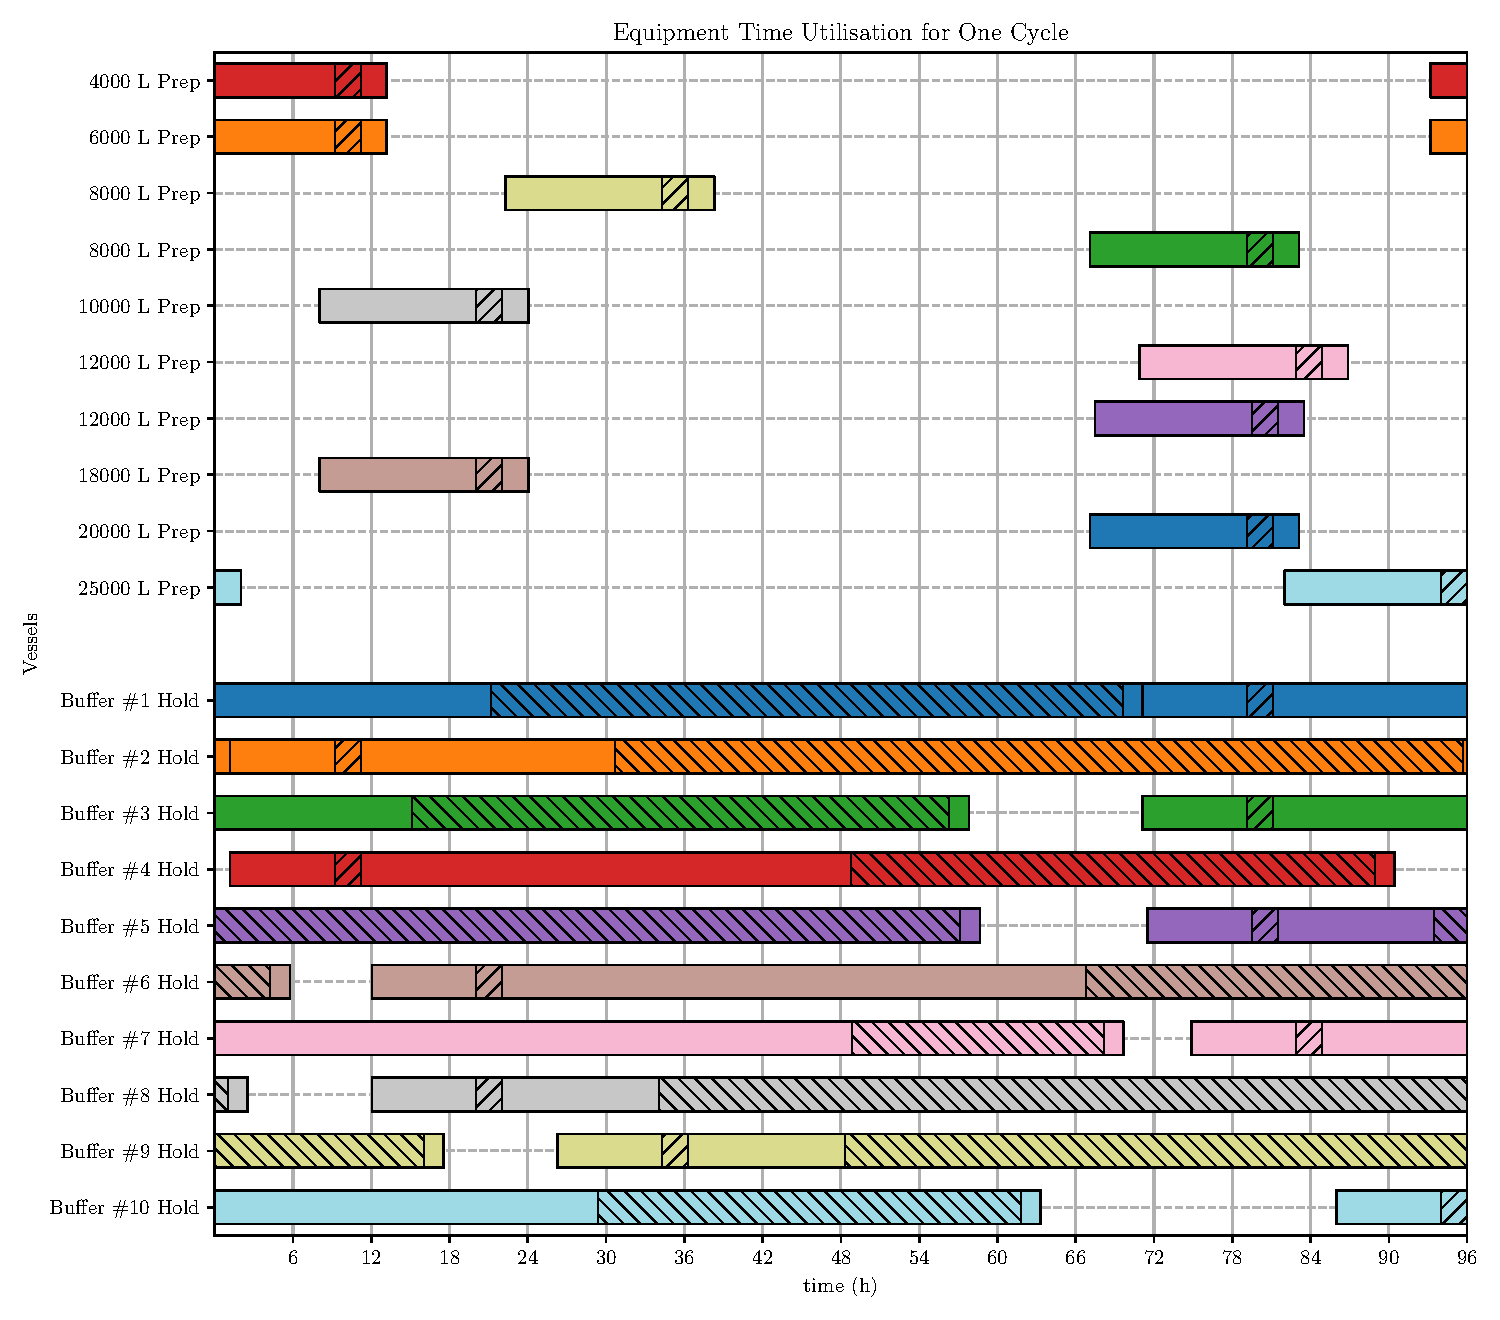
\includegraphics[angle=0,scale=0.55]{../examples/large-scale/plot1.pdf}
    \caption{Large-Scale Example -- Primary Objective}
    \label{fig.primary}
\end{figure}

Note that the solution requires four vessels, with volumes of
\SI{8000}{\litre}, \SI{10000}{\litre}, \SI{15000}{\litre} and
\SI{20000}{\litre} respectively.  
Recall that one of our decision variables is $\boldsymbol{z}_{n}$, the buffer
hold duration.
In the figure below, buffers \#5, \#8 and \#9 are scheduled such that their 
hold procedures are bottlenecked, i.e. the start of the hold procedure for one
cycle coincides with the end of the hold procedure for the previous cycle.
For each of these three buffers, it can also be seen that there exists some
free time after each of their respective preparation procedures.
Delaying the preparation of each of these three buffers by e.g. 1 hour would
also give an optimal solution, with the vessel selection unchanged.
Note that delaying a preparation by some amount $\delta$ is equivalent to 
reducing $\boldsymbol{z}_{n}$ by $\delta$.
Recall also that $\boldsymbol{z}_{n}$ has a lower bound, 
$\Delta t_{\mathit{HOLD,MIN}}$.
In terms of visualising a realistic schedule, it is desirable to minimise the
hold durations, i.e. we wish to define a new objective function, to be
minimised:
\begin{equation}
    \boldsymbol{Y} = \sum_{n \in N} \boldsymbol{z}_{n} \quad \forall n \in N
    \label{eq.objfn2}
\end{equation}
Note that we want to maintain the original optimum objective function value,
i.e. we define
\begin{equation}
    Z^{\prime} = \min \boldsymbol{Z}
\end{equation}
In the above equation, $Z^{\prime}$ is the optimal objective function value obtained by solving
the complete model.
Note that $Z^{\prime}$ is not bolded, as it is treated as a constant parameter
in our second-pass model.
The complete model is then re-run with the original objective function replaced
by the new objective, $\min \boldsymbol{Y}$, with the following constraint
added:
\begin{equation}
    \sum_{m \in M} \sum_{p \in P} c_m \boldsymbol{y}_{mp} = Z^{\prime}
    \label{eq.constr10}
\end{equation}

Implementing the secondary goal programming model on the same data-set yields
the following plot.
Note that the buffer hold procedures for buffers \#5, \#8 and \#9 are no longer
bottlenecked.
Note also that, although the same preparation vessels are selected (i.e. the
same minimal cost is obtained), some buffers are now prepared in different
vessels to those originally assigned.
For example, in the original result, buffer \#8 was prepared in a 15,000 l
vessel and with the secondary goal added, it is prepared in am 8,000 l vessel.

\begin{figure}
    \centering
    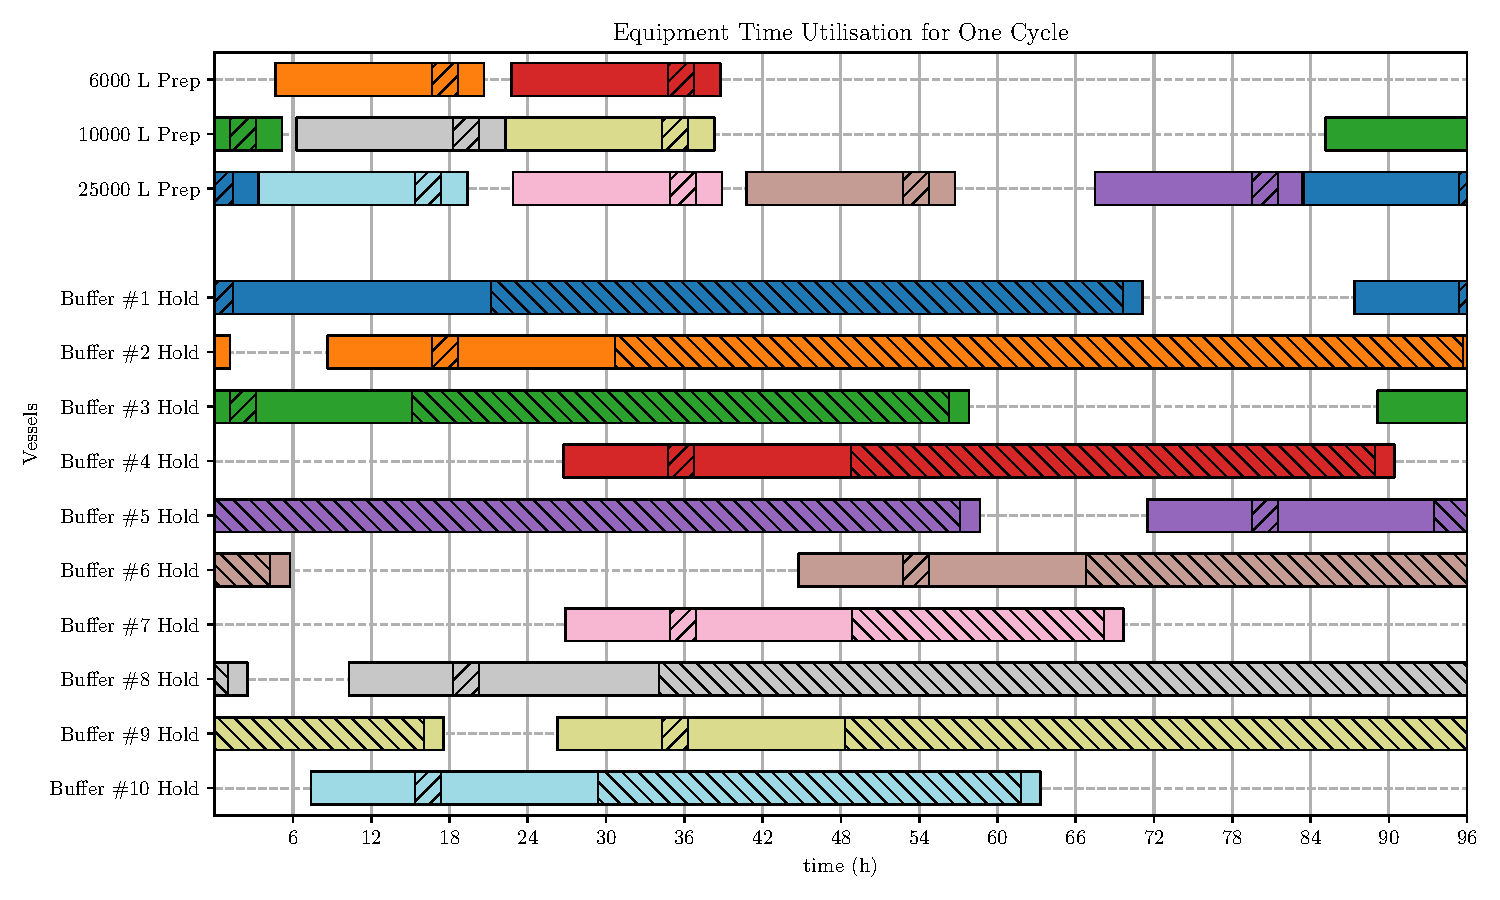
\includegraphics[angle=0,scale=0.55]{../examples/large-scale/plot2.pdf}
    \caption{Large-Scale Example -- Secondary Objective}
    \label{fig.secondary}
\end{figure}

\subsection{Secondary Model Summary}\label{SS.model2summary}

The secondary model is summarised below:

Minimise:
\begin{equation}
    \boldsymbol{Y} = \sum_{n \in N} \boldsymbol{z}_{n} \quad \forall n \in N
    \tag{\ref{eq.objfn2}}
\end{equation}
Subject to:
\begin{equation}
    \sum_{p \in P} \boldsymbol{x}_{np} = 1 \quad \forall n \in N
    \tag{\ref{eq.constr1}}
\end{equation}
\begin{equation}
    \sum_{m \in M} \boldsymbol{y}_{mp} \le 1 \quad \forall p \in P
    \tag{\ref{eq.constr2}}
\end{equation}
\begin{equation}
    U_{n} \boldsymbol{x}_{np} - \sum_{m \in M} V_{m} \boldsymbol{y}_{mp} \le 0
    \quad \forall n \in N, \quad \forall p \in P
    \tag{\ref{eq.constr3a}}
\end{equation}
\begin{equation}
    V_{\mathit{MAX}} \boldsymbol{x}_{np} + r_{\mathit{MINFILL}} \sum_{m \in M}
    V_{m} \boldsymbol{y}_{mp} \le U_{n} + V_{\mathit{MAX}} \quad \forall n \in
    N, \quad \forall p \in P
    \tag{\ref{eq.constr3b}}
\end{equation}
\begin{equation}
    \Delta t_{\mathit{PREP,TOTAL}} \sum_{n \in N} \boldsymbol{x}_{np} \le 
    r_{\mathit{UTIL}} \lambda \quad \forall p \in P
    \tag{\ref{eq.constr4}}
\end{equation}
\begin{equation}
    \boldsymbol{z}_{n} \le \lambda - \left( \Delta t_{\mathit{HOLD,PRE}} +
    \Delta t_{\mathit{TRANSFER}} + \Delta t_{\mathit{USE},n} + \Delta
    t_{\mathit{HOLD,POST}} \right) \quad \forall n \in N
    \tag{\ref{eq.constr5}}
\end{equation}
\begin{equation}
    \begin{split}
        \begin{alignedat}{3}
            \boldsymbol{x}_{np} & {}+{} & \boldsymbol{x}_{kp} & {}-{} & 2
            \boldsymbol{w}_{nkp} & \ge 0\\
            \boldsymbol{x}_{np} & {}+{} & \boldsymbol{x}_{kp} & {}-{} &
            \boldsymbol{w}_{nkp} & \le 1\\
        \end{alignedat}
    \end{split}
    \quad\quad
    \begin{split}
        \forall n \in N, \quad \forall k \in N, k > n
    \end{split}
    \tag{\ref{eq.constr6}}
\end{equation}
\begin{equation}
    \sum_{p \in P} \boldsymbol{w}_{nkp} - \boldsymbol{v}_{nk} \le 0 \quad
    \forall n \in N, \quad \forall k \in N, k > n
    \tag{\ref{eq.constr7}}
\end{equation}
\begin{equation}
    \begin{split}
        \begin{alignedat}{2}
            \boldsymbol{z}_{n} & {}-{} & \lambda \boldsymbol{q}_{n} & \le
            t_{\mathit{USE},n}^{*}\\
            \boldsymbol{z}_{n} & {}-{} & \lambda \boldsymbol{q}_{n} & \ge
            t_{\mathit{USE},n}^{*} - \lambda
        \end{alignedat}
    \end{split}
    \quad\quad
    \begin{split}
        \forall n \in N
    \end{split}
    \tag{\ref{eq.constr8a}}
\end{equation}
\begin{equation}
    \begin{split}
        \boldsymbol{z}_{n} - \boldsymbol{z}_{k} - \lambda \boldsymbol{q}_{n}
        + \lambda \boldsymbol{q}_{k} + \lambda \boldsymbol{u}_{nk} &\ge
        t_{\mathit{USE},n}^{*} - t_{\mathit{USE},k}^{*}\\
        \boldsymbol{z}_{n} - \boldsymbol{z}_{k} - \lambda \boldsymbol{q}_{n}
        + \lambda \boldsymbol{q}_{k} + \lambda \boldsymbol{u}_{nk} &\le
        t_{\mathit{USE},n}^{*} - t_{\mathit{USE},k}^{*} + \lambda\\
        \forall n \in N, \quad \forall k \in N, k > n
    \end{split}
    \tag{\ref{eq.constr8b}}
\end{equation}
\begin{equation}
    \begin{split}
        \begin{alignedat}{10}
            &\boldsymbol{z}_{n} {}-{} &\boldsymbol{z}_{k} {}+{} &2 \lambda
            \boldsymbol{u}_{nk} {}-{} &2 \lambda \boldsymbol{v}_{nk} &\ge
            &t_{\mathit{USE},n}^{*} {}-{} &t_{\mathit{USE},k}^{*} {}+{}
            &\Delta &t_{\mathit{PREP,TOTAL}} {}-{} 2 &\lambda\\
            - &\boldsymbol{z}_{n} {}+{} &\boldsymbol{z}_{k} {}-{} &2 \lambda
            \boldsymbol{u}_{nk} {}-{} &2 \lambda \boldsymbol{v}_{nk} &\ge
            - &t_{\mathit{USE},n}^{*} {}+{} &t_{\mathit{USE},k}^{*} {}+{}
            &\Delta &t_{\mathit{PREP,TOTAL}} {}-{} 4 &\lambda
        \end{alignedat}
        \\\forall n \in N, \quad \forall k \in N, k > n
    \end{split}
    \tag{\ref{eq.constr9}}
\end{equation}
\begin{equation}
    \sum_{m \in M} \sum_{p \in P} c_m \boldsymbol{y}_{mp} = Z^{\prime}
    \tag{\ref{eq.constr10}}
\end{equation}
Where:
\begin{equation}
    \boldsymbol{q}_{n} \in \left\{ 0, 1 \right\} \quad \forall n \in N
    \tag{\ref{eq.q}}
\end{equation}
\begin{equation}
    \boldsymbol{u}_{nk} \in \left\{ 0, 1 \right\} \quad \forall n \in N \quad
    \forall k \in N
    \label{eq.u}
\end{equation}
\begin{equation}
    \boldsymbol{v}_{nk} \in \left\{ 0, 1 \right\} \quad \forall n \in N \quad
    \forall k \in N
    \tag{\ref{eq.v}}
\end{equation}
\begin{equation}
    \boldsymbol{w}_{nkp} \in \left\{ 0, 1 \right\} \quad \forall n \in N \quad
    \forall k \in N \quad \forall p \in P
    \tag{\ref{eq.w}}
\end{equation}
\begin{equation}
    \boldsymbol{x}_{np} \in \left\{ 0, 1 \right\} \quad \forall n \in N \quad
    \forall p \in P
    \tag{\ref{eq.x}}
\end{equation}
\begin{equation}
    \boldsymbol{y}_{mp} \in \left\{ 0, 1 \right\} \quad \forall m \in M \quad
    \forall p \in P
    \tag{\ref{eq.y}}
\end{equation}
\begin{equation}
    \Delta t_{\mathit{HOLD,MIN}} \le \boldsymbol{z}_{n} \le \Delta
    t_{\mathit{HOLD,MAX}}; \quad \boldsymbol{z}_{n} \in \mathbb{R} \quad
    \forall n \in N
    \tag{\ref{eq.z}}
\end{equation}


\section{Implementation}\label{S.implementation}

\subsection{Code and APIs etc}\label{SS.completesummary}

\subsection{Plotting}\label{SS.completesummary}
